\documentclass[11pt, a4paper]{article}
\usepackage[utf8]{inputenc}
\usepackage[margin=1in]{geometry}
\usepackage[toc, page]{appendix}
\usepackage{multirow}
\usepackage{pdflscape}
\usepackage{array}
\usepackage{longtable}
\usepackage{color} 
\usepackage[pdftex]{hyperref}
\hypersetup{
	colorlinks=true,
	linktoc=all,
	linkcolor=black,
	citecolor=black,
}
\usepackage[export]{adjustbox}
\usepackage{float}
\restylefloat{table}
\usepackage{array}
\usepackage[final]{microtype}
\usepackage{tikz}
\usepackage{graphicx}
\usepackage{pgfplots}
\pgfplotsset{compat=newest}
\usepackage{filecontents}
\usepackage{multirow}
\usepackage{callouts}
\usepackage{longtable}
\usepackage{array}
\usepackage[justification=centering]{caption} 
\usetikzlibrary{intersections}
\usepackage{fontawesome}
\usepackage{capt-of}
\usepackage{setspace}
\usepackage{tablefootnote}
\usepackage{subcaption}
\usepackage{caption}
\captionsetup[figure]{font=footnotesize}
\captionsetup[table]{font=footnotesize}
\usepackage{wrapfig}
\usepackage{scrextend}
\usepackage[normalem]{ulem}
\usepackage{caption}
\usepackage{textcomp}
\useunder{\uline}{\ul}{}
\deffootnote{0em}{1.6em}{\thefootnotemark.\enskip}
\newcommand{\roundpic}[4][]{
  \tikz\node [circle, minimum width = #2,
    path picture = {
      \node [#1] at(path picture bounding box.center) {
        \includegraphics[width=#3]{#4}};
    }] {};}
    \newcolumntype{P}[1]{>{\centering\arraybackslash}p{#1}}


\def\x{\roundpic[xshift=0cm,yshift=0cm]{1.75cm}{1.75cm}{Frank_Tang.png}}
\def\y{\parbox[t]{2.5in}{\includegraphics[width=0.7cm]{Bar.png} \\ \textbf{Frank Tang in Beijing}\\ {Published: 2:58 pm, 8 May, 2020}}}
\def\z{\parbox[t]{5.3in}{\includegraphics[width=0.7cm]{Bar.png} \\ \textbf{Frank Tang}\\ {Frank Tang joined the SCMP in 2016 after a decade of China economy coverage and government policy analysis.}}}

\title{MYP Economics G2 01 - Macroeconomics Commentary}
\author{Adithya Narayanan}
\date{15 May, 2020}

\begin{document}
	\begin{titlepage}
		\maketitle

		\begin{center}
			\large How has the Chinese economy been affected by, and is responding to COVID-19

			Word count: 748
		\end{center}
		\thispagestyle{empty}
	\end{titlepage}
	
	\newpage
	\tableofcontents
	\thispagestyle{empty}
	\newpage
	\clearpage
	\setcounter{page}{1}
	\setcounter{secnumdepth}{0}
    \section{Article:}
        \textbf{Economy/China Economy}

        \bigbreak
		\noindent
        \textbf{\LARGE Explainer | China coronavirus stimulus: what measures have been used to combat the economic impact of Covid-19?}
        
        \begin{itemize}
            \item Faced with the unprecedented economic impact of the coronavirus outbreak, China has rolled out numerous measures to aid the world’s second largest economy

            \item In response to the global financial crisis in 2008, China implemented a massive 4 trillion yuan(US\$564 billion) stimulus package
        \end{itemize}
        
        \vspace{-6mm}

        \begin{figure}[H]
            \ \ \raisebox{\baselineskip -\heightof{\x}}{\x} 
            ~\y
        \end{figure}

        \vspace{-8mm}
        
        \begin{figure}[H]
            \includegraphics[width=6.27in]{Title_image.jpg}
            \caption*{With the coronavirus posing a greater threat to the economy, the outbreak left the top leadership with a decision to make, as the efforts in 2008 left the nation with a mountain of debt. Photo: Bloomberg}
        \end{figure}

        In response to the global financial crisis in 2008, China rolled out a massive 4 trillion yuan(US\$564 billion) stimulus package.
        \bigbreak
        With the coronavirus posing an even greater threat to the economy, the outbreak left the top leadership with a decision to make, as the efforts in 2008 also left the nation with a mountain of debt.
        \bigbreak
        Before the outbreak, China had already cut the top tier of the value-added tax(VAT) rate to 13 per cent from 16 per cent in April 2019, after a one percentage point cut in 2018. It had also raised the personal income tax threshold by 1,500 yuan(US\$211) to 5,000 yuan(US\$705) in January 2019, while allowing more pre-tax deduction in terms of child care, elderly care, medical expenditure, mortgage interest rates and continued learning. The total tax cuts amounted to 2.3 trillion yuan(US\$324 billion) in 2019.
        \bigbreak
        These moves were largely in response to the trade war with the United States, which led China’s economy last year to slow to a growth rate of 6.1 per cent, the slowest rate since political turmoil ravaged the country in 1990.
        \bigbreak
        Here, we track China’s response to the coronavirus outbreak, which emerged just as those trade war tensions with the US appeared to have cooled with the signing of the phase one deal in January.
        \subsection{Coronavirus cases}
            \begin{table}[H]
                \centering
                \begin{tabular}{|P{7.96cm}|P{7.96cm}|}
                    \hline
                    \multicolumn{2}{|c|}{\textbf{\Large \strut 4,348,507}}\\
                    \multicolumn{2}{|c|}{\small Confirmed Covid-19 cases}\\
                    \hline
                    \textbf{\Large \strut 297,207} & \textbf{\Large 1,548,375}\\
                    \small total deaths & \small total recovered\\
                    \hline
                \end{tabular}
            \end{table} 

            \vspace{-10mm}

            \begin{table}[H]
                \centering
                \begin{tabular}{p{7.96cm}P{3.98cm}P{3.98cm}}
                    & Cases & Deaths\\
                    \hline
                    United States & 1,390,764 & 84,136\\
                    \hline
                    Russia & 242,271 & 2,212\\
                    \hline
                    United Kingdom & 230,986 & 33,264\\
                    \hline
                    Spain & 228,691 & 27,104\\
                    \hline
                    Italy & 222,104 & 31,106\\
                    \hline
                \end{tabular}
                \caption*{Last updated: 14 May, 06:00PM \\
                Sources: Johns Hopkins University, WHO and health authorities}
            \end{table} 

            \textbf{May 14, 2020 – China requires greater budget support, finance minister says}
            \bigbreak
            Finance Minister Liu Kun says China will increase fiscal expenditure in 2020 to help offset the damage to the economy resulting from the coronavirus outbreak and ensure that the nation can reduce poverty and achieve its target of building up a comprehensively well-off society by the end of the year.
            \bigbreak
            China also announces a decision to waive the value-added tax(VAT) and some fees on certain film-related businesses until the end of 2020.
            \bigbreak
            \noindent
            \textbf{\Large April 29, 2020 – China announces National People’s Congress will resume on May 22}
            \bigbreak
            \noindent
            \textbf{April 24, 2020 – PBOC cuts MLF rate}
            \bigbreak
            People’s Bank of China(PBOC) cuts its targeted medium-term lending facility(MLF) rate by 20 basis points to 2.95 per cent, injecting 56.1 billion yuan(US\$7.9 billion) into the banking system.
            \bigbreak
            \noindent
            \textbf{April 21, 2020 – China extends welfare support to vast migrant labour force}
            \bigbreak
            China’s State Council announces a new package of welfare support to help vulnerable migrant workers.
            \bigbreak
            Under the move, state-funded infrastructure projects will be able to use up to 15 per cent of investment for a project to pay wages in an effort to expand hiring. Previously only 10 per cent was earmarked for salaries.
            \bigbreak

        \subsection{China's GDP growth, quarterly}

            \begin{figure}[H]
                \includegraphics[width=6.27in]{GDP_Growth.png}
                \caption*{Source: National Bureau of Statistics}
            \end{figure}

            The State Council also urges local authorities to provide unemployment benefits or “minimum living guarantees” to migrant workers, who had not previously been covered.
            \bigbreak
            The reserve coverage ratio as required by Chinese regulators will also be reduced by 20 basis points, to unleash more funds for micro and small-enterprises. The previous reserve coverage ratio required of Chinese banks was between 120 per cent and 150 per cent, with the reduction meaning that some small and medium-sized banks could see this figure drop to as low as 100 per cent.
            \bigbreak
            \noindent
            \textbf{April 20, 2020 – China lowers loan prime rate}
            \bigbreak
            China lowers its one-year loan prime rate(LPR) by 20 basis points to 3.85 per cent, while the five-year LPR is cut by 10 basis points to 4.65 per cent.
            \bigbreak
            \noindent
            \textbf{\Large April 17, 2020 – China's economy shrinks 6.8 per cent in first quarter}
            \bigbreak
            \noindent
            \textbf{April 15, 2020 – China cuts MLF borrowing costs to record low}
            \bigbreak
            People’s Bank of China(PBOC) lowers the interest rate on its one-year medium-term lending facility(MLF) loans to financial institutions to 2.95 per cent, down 20 basis points from 3.15 per cent.
            \bigbreak
            \noindent
            \textbf{April 14, 2020 – Special purpose bonds for infrastructure projects}
            \bigbreak
            China’s State Council’s authorises a further 1 trillion yuan(US\$140 billion) in local government special purpose bonds for infrastructure projects. It also doubles funding for old neighbourhood reconstruction programmes and extends the 15 per cent preferential income tax rate for some investments in western regions.
            \bigbreak
            \noindent
            \textbf{\Large April 8, 2020 – Wuhan lockdown ends}
            \bigbreak
            \noindent
            \textbf{April 7, 2020 – New pilot zones}
            \bigbreak
            China’s State Council’s executive meeting chaired by Premier Li Keqiang announces plans to build 46 new integrated pilot zones for cross-border e-commerce around the country.
            \bigbreak
            The country will also extend some expired preferential tax policies to the end of 2023 to help small and micro-sized businesses, self-employed individuals and farmers. Under the policies, small and micro enterprises, as well as rural households, are exempted from the replacement of interest income on loans of 1 million yuan(US\$141,000) and below.
            \bigbreak
            \textbf{April 3, 2020 – RRR cut to aid SMEs}
            \bigbreak
            People’s Bank of China(PBOC) announces reserve requirement ratio(RRR) cuts for rural banks and some city commercial banks totalling 100 basis points, which is expected to release around 400 billion yuan(US\$57 billion) of funds into the banking system. The cuts of 50 basis points each time will be made on April 15 and May 15. After the cuts, the RRR for the country's small and medium-sized lenders will be slashed to 6 per cent.
            \bigbreak
            Some China-made coronavirus test kits and face masks rejected as ‘unreliable’ in European countries
            \bigbreak
            \noindent
            \textbf{March 31, 2020 – State Council rolls out host of measures}
            \bigbreak
            China’s State Council rolls out a host of measures to support the economy, including an additional central bank credit line of 1 trillion yuan(US\$140 billion) to small lenders. The government also announces new monetary policies, including the prospect of lower deposit reserve requirements for small banks in the future and an additional 1 trillion yuan for small banks to spur lending to small businesses.
            \bigbreak
            It also authorises a third batch of local government bond issuance this year to support “effective investments” in areas from affordable housing to motorways. The State Council did not elaborate on the size of the bond issuance – which follows previous batches worth 1 trillion yuan in November and 290 billion yuan(US\$41 billion) in February – but urged local governments to sell them by the end of June.
            \bigbreak
            Beijing will also extend subsidies and purchase tax exemptions for new energy vehicles like electric and hybrid cars until the end of 2022.
            \bigbreak
            The central government will double the temporary monthly allowance for low-income families between March and June to counter price increases caused by the coronavirus outbreak.

        \subsection{Coronavirus in context:}
            \begin{figure}[H]
                \includegraphics[width=6.27in]{Corona_in_context.png}
                \caption*{
                    Source: China's NHC, state media, other authorities\\
                    *US Centers for Disease Control and Prevention(CDC) estimated data from 2019-20 Season}
            \end{figure}
            \bigbreak

            \textbf{March 30, 2020 – Reverse repo rate cut}
            \bigbreak
            People’s Bank of China(PBOC) lowers the seven-day reverse repurchase agreement rate(RRR) by 20 basis points to 2.2 per cent, injecting 50 billion yuan(US\$7 billion) into the market. Before the move, China’s central bank had skipped reverse repos for 29 straight trading days.
            \bigbreak
            \noindent
            \textbf{March 27, 2020 – China responds to G20 pledge}
            \bigbreak
            China’s State Council says it is ready to raise its budget deficit above 3 per cent of gross domestic product(GDP) after the Group of 20(G20) pledges a US\$5 trillion economic rescue package.
            \bigbreak
            \noindent
            \textbf{\Large March 26, 2020 – G20 leaders pledge US\$5 trillion fiscal stimulus package}
            \bigbreak
            \noindent
            \textbf{March 16, 2020 – Further RRR cut}
            \bigbreak
            People’s Bank of China(PBOC) pumps 550 billion yuan(US\$78 billion) into its banking system to spur additional lending to factories and households by cutting banks' reserve requirement ratio(RRR) by 50 or 100 basis points, with the exact cut based on individual assessments.
            \bigbreak
            \noindent
            \textbf{March 14, 2020 – First city to distribute vouchers}
            \bigbreak
            Nanjing is the first Chinese city to grant 300 million yuan(US\$42 million) of consumer vouchers aimed at improving spending.
            \bigbreak
            \noindent
            \textbf{\Large March 11, 2020 – World Health Organisation(WHO) declares coronavirus a pandemic}
            \bigbreak
            \noindent
            \textbf{March 3, 2020 – Harbour, port fees cut}
            \bigbreak
            China’s State Council cuts harbour construction fees and lowers other port related fees by 20 per cent from March to June. It also increases provincial governments' share of overall tax revenue by 5 percentage points, with an estimated 110 billion yuan(US\$15.5 billion) allocated to county-level governments. Fiscal transfer payments from the central government are also accelerated .
            \bigbreak
            \noindent
            \textbf{February 25, 2020 – National People’s Congress formally postponed}
            \bigbreak
            \noindent
            \textbf{\Large February 25, 2020 – Help for small businesses, rural areas, farms, agriculture firms}
            \bigbreak
            China’s State Council approves an additional 500 billion yuan(US\$70 billion) for small business lending on top of 300 billion yuan approved earlier in February. Certain small businesses will also be able to to postpone loan repayments.
            \bigbreak
            To help spur borrowing, the official interest rate set by the central bank for commercial lenders extending credit to rural areas, farms and agriculture firms, as well as other small businesses, was cut by a quarter of a percentage point to 2.5 per cent. Regional banks that extend such loans at a rate no higher than a half percentage point above the benchmark loan prime rate(LPR) will also be eligible to apply for the new government funding.
            \bigbreak
            The State Council also orders large state-owned banks to increase lending to small businesses by at least 30 per cent in the first half of 2020. China’s three government-run policy banks were also told to lend 350 billion yuan(US\$50 billion) to small businesses at preferential rates.
            \bigbreak
            \noindent
            \textbf{February 22, 2020 – Cheaper electricity}
            \bigbreak
            China’s state planner, the National Development and Reform Commission(NDRC), lowers companies’ electricity price by 5 per cent from February 1 to June 30, except high energy consuming industries.
            \bigbreak
            \noindent
            \textbf{February 20, 2020 – Loan rate cut}
            \bigbreak
            The People’s Bank of China lowers the one-year loan prime rate(LPR) by 10 basis points to 4.05 per cent. The five-year LPR was also lowered by five basis points to 4.75 per cent.
            \bigbreak
            \noindent
            \textbf{February 18, 2020 – Pension fund contribution}
            \bigbreak
            China’s State Council allows businesses to reduce or even stop contributions to provincial pension funds as well as unemployment and work insurance from February to June. It also halves the social contribution rate for large corporations between February and April. Companies can also apply for the postponement of housing fund contributions before the end of June.
            \bigbreak
            \noindent
            \textbf{February 5, 2020 – VAT exemption, loan subsidies}
            \bigbreak
            China’s State Council exempts transport and virus control companies from value-added tax(VAT), creates subsidies for loans to pandemic control companies and suspends requirements for civil aviation companies to pay into the civil aviation development fund.
            \bigbreak
            \noindent
            \textbf{February 3, 2020 – Open market operations, reverse repo cut}
            \bigbreak
            On the first day the stock markets in Shanghai and Shenzhen reopened after the Lunar New Year holiday, the People’s Bank of China(PBOC) injects 1.2 trillion yuan(US\$170 billion) of liquidity through reverse bond repurchase agreements. It also lowers the seven-day reverse repurchase agreement rate(RRR) by 10 basis points to 2.40 per cent from 2.50 per cent, while also cutting the 14-day tenor to 2.55 per cent from 2.65 per cent.
            \bigbreak
            \noindent
            \textbf{February 1, 2020 – Coronavirus-relief bonds}
            \bigbreak
            The People’s Bank of China(PBOC) and the China Banking and Insurance Regulatory Commission(CBIRC) allows the sale of coronavirus-relief bonds by financial institutions.
            \bigbreak
            \noindent
            \textbf{January 30, 2020 – Help for front line medical staff, party members}
            \bigbreak
            The Organisation Department of the Communist Party of China allocates 108 million yuan(US\$15 million) to help front line medical personnel, as well as grass roots-level Communist Party members.
            \bigbreak
            \noindent
            \textbf{January 27, 2020 – Hospital construction}
            \bigbreak
            China’s National Development and Reform Commission(NDRC) allocates 300 million yuan(US\$42 million) to fund the construction of two temporary coronavirus hospitals in Wuhan.
            \bigbreak
            \noindent
            \textbf{\Large January 23, 2020 – Wuhan lockdown begins}
            \bigbreak
            \noindent
            \textbf{\Large January 11, 2020 – China reports first coronavirus-related death}
            \bigbreak
            \noindent
            \textbf{January 6, 2020 – Reserve ratio cut}
            \bigbreak
            People’s Bank of China(PBOC) cuts banks’ reserve ratio requirement(RRR) by 0.5 percentage points. The RRR – the money that banks are required to hold in reserve – for big banks is lowered to 12.5 per cent, while the ratio for small and medium-sized banks is reduced to 10.5 per cent and 7 per cent respectively.
            \bigbreak
            \noindent
            \textbf{\Large December 31, 2019 – First report of a ‘mystery illness’ in Wuhan}
            \begin{figure}[H]
                \raisebox{\baselineskip -\heightof{\x}}{\x} 
                ~\z
            \end{figure}
            \newpage
    \section{Commentary:}
        \begin{center}
            \textbf{\Large How has the Chinese economy been affected by, and is responding to COVID-19}
        \end{center}
        The effect of COVID-19 has been rather drastic on China's economy, and as such, equally drastic measures have been implemented and discussed below, to combat the economic effect of COVID-19.

        \subsection{Effect of COVID-19 on the Chinese economy:}
                        
            \begin{figure}[H]
                \centering
                \begin{tikzpicture}[x=0.75pt,y=0.75pt,yscale=-1,xscale=1]
                        %uncomment if require: \path(0,459); %set diagram left start at 0, and has height of 459
            
                        %Straight Lines [id:da44765396271940605] 
                        \draw   (185,376) --(498.5,376) ;
                        \draw [shift={(500.5,376)}, rotate = 180] [color={rgb, 255:red, 0; green, 0; blue, 0 }  ][line width=0.75]   (10.93,-3.29) .. controls(6.95,-1.4) and(3.31,-0.3) ..(0,0) .. controls(3.31,0.3) and(6.95,1.4) ..(10.93,3.29)   ;
                        %Straight Lines [id:da5202556406249792] 
                        \draw   (185,376) --(185,62.06) ;
                        \draw [shift={(185,60.06)}, rotate = 450] [color={rgb, 255:red, 0; green, 0; blue, 0 }  ][line width=0.75]   (10.93,-3.29) .. controls(6.95,-1.4) and(3.31,-0.3) ..(0,0) .. controls(3.31,0.3) and(6.95,1.4) ..(10.93,3.29)   ;
                        %Straight Lines [id:da9136007481866493] 
                        \draw   (186,265) --(449.5,265) ;
                        %Curve Lines [id:da768389471708891] 
                        \draw   (424.5,265.06) .. controls(446.5,264.12) and(443.5,252.06) ..(444,234.06) ;
                        %Straight Lines [id:da02274241573453284] 
                        \draw   (469,110.06) --(469,234) ;
                        %Straight Lines [id:da6749686149209355] 
                        \draw   (444,111.06) --(444,234.06) ;
                        %Straight Lines [id:da7534024269886006] 
                        \draw   (466,131) --(448.5,131) ;
                        \draw [shift={(446.5,131)}, rotate = 360] [color={rgb, 255:red, 0; green, 0; blue, 0 }  ][line width=0.75]   (10.93,-3.29) .. controls(6.95,-1.4) and(3.31,-0.3) ..(0,0) .. controls(3.31,0.3) and(6.95,1.4) ..(10.93,3.29)   ;
                        %Straight Lines [id:da2688494908989494] 
                        \draw   (421,171) --(492.5,350.06) ;
                        %Straight Lines [id:da8697542263375846] 
                        \draw   (352,171) --(423.5,350.06) ;
                        %Straight Lines [id:da9607338968630843] 
                        \draw   (410.5,179) --(367.5,179) ;
                        \draw [shift={(365.5,179)}, rotate = 360] [color={rgb, 255:red, 0; green, 0; blue, 0 }  ][line width=0.75]   (10.93,-3.29) .. controls(6.95,-1.4) and(3.31,-0.3) ..(0,0) .. controls(3.31,0.3) and(6.95,1.4) ..(10.93,3.29)   ;
                        %Straight Lines [id:da278493289337407] 
                        \draw  [dashed] (183.5,261.53) --(456.75,261.53) ;
                        %Straight Lines [id:da7029207353305877] 
                        \draw  [dashed] (456.75,375.06) --(456.75,261.53) ;
                        %Straight Lines [id:da3501351654583038] 
                        \draw  [dashed] (389.75,377.06) --(389.75,267.06) ;
                        %Curve Lines [id:da08385215118747169] 
                        \draw   (449.5,265) .. controls(471.5,264.06) and(468.5,252) ..(469,234) ;
                        %Shape: Circle [id:dp88931796784892] 
                        \draw  [draw opacity=0][fill={rgb, 255:red, 0; green, 0; blue, 0 }  ,fill opacity=1 ](455.28,264) .. controls(455.28,262.64) and(456.39,261.53) ..(457.75,261.53) .. controls(459.11,261.53) and(460.22,262.64) ..(460.22,264) .. controls(460.22,265.36) and(459.11,266.47) ..(457.75,266.47) .. controls(456.39,266.47) and(455.28,265.36) ..(455.28,264) -- cycle ;
                        %Shape: Circle [id:dp09002438261461232] 
                        \draw  [draw opacity=0][fill={rgb, 255:red, 0; green, 0; blue, 0 }  ,fill opacity=1 ](387.28,265.59) .. controls(387.28,264.23) and(388.39,263.12) ..(389.75,263.12) .. controls(391.11,263.12) and(392.22,264.23) ..(392.22,265.59) .. controls(392.22,266.95) and(391.11,268.06) ..(389.75,268.06) .. controls(388.39,268.06) and(387.28,266.95) ..(387.28,265.59) -- cycle ;
                        %Straight Lines [id:da24913817983365516] 
                        \draw   (155.5,256) --(155.5,272.06) ;
                        \draw [shift={(155.5,274.06)}, rotate = 270] [color={rgb, 255:red, 0; green, 0; blue, 0 }  ][line width=0.75]   (10.93,-3.29) .. controls(6.95,-1.4) and(3.31,-0.3) ..(0,0) .. controls(3.31,0.3) and(6.95,1.4) ..(10.93,3.29)   ;
                        %Straight Lines [id:da5756014791745612] 
                        \draw   (455,398.06) --(392.3,398.06) ;
                        \draw [shift={(390.3,398.06)}, rotate = 360] [color={rgb, 255:red, 0; green, 0; blue, 0 }  ][line width=0.75]   (10.93,-3.29) .. controls(6.95,-1.4) and(3.31,-0.3) ..(0,0) .. controls(3.31,0.3) and(6.95,1.4) ..(10.93,3.29)   ;
            
                        \draw(174,376) node [anchor=north west][inner sep=0.75pt]   [align=left] {0};
                        % Text Node
                        \draw(494,344) node [anchor=north west][inner sep=0.75pt]  [font=\small] [align=left] {$AD_1$};
                        % Text Node
                        \draw(425,343) node [anchor=north west][inner sep=0.75pt]  [font=\small] [align=left] {$AD_2$};
                        % Text Node
                        \draw(470,92) node [anchor=north west][inner sep=0.75pt]  [font=\small] [align=left] {$AS_1$};
                        % Text Node
                        \draw(415,92) node [anchor=north west][inner sep=0.75pt]  [font=\small] [align=left] {$AS_2$};
                        % Text Node
                        \draw(480,381) node [anchor=north west][inner sep=0.75pt]   [align=left] {Total output \\(Real GDP, USD, trillions)};
                        % Text Node
                        \draw(82,75) node [anchor=north west][inner sep=0.75pt]   [align=left] {Price Level(¥)};
                        % Text Node
                        \draw(465,262) node [anchor=north west][inner sep=0.75pt]  [font=\footnotesize] [align=left] {a};
                        % Text Node
                        \draw(378,269) node [anchor=north west][inner sep=0.75pt]  [font=\footnotesize] [align=left] {b};
                        % Text Node
                        \draw(162,249) node [anchor=north west][inner sep=0.75pt]  [font=\small] [align=left] {$Pl_e$};
                        % Text Node
                        \draw(162,267) node [anchor=north west][inner sep=0.75pt]  [font=\small] [align=left] {$Pl_2$};
                        % Text Node
                        \draw(447,378.06) node [anchor=north west][inner sep=0.75pt]  [font=\small] [align=left] {2.8};
                        % Text Node
                        \draw(380,378.06) node [anchor=north west][inner sep=0.75pt]  [font=\small] [align=left] {2.6};
                        
                        \draw(409,400.06) node [anchor=north west][inner sep=0.75pt]  [font=\footnotesize] [align=left] {\mbox{-}6.8\%};
            
                    \end{tikzpicture}
                \caption{Narayanan, Adithya. \textit{Effect of COVID-19 on the Chinese economy in the first quarter of 2020}}
            \end{figure}
            
            The onset of the COVID-19 pandemic, resulted in lower consumer expenditure, investment by firms and net exports. Reduction in consumption can be attributed to reductions in disposable income as individuals are forced to take wageless leave or become unemployed, caused by lower derived demand for labour from lower consumer expenditure. Reductions in investment occur as firms face reduced demand, also resulting in lower net exports. As such, the Aggregate Demand(AD), defined as ``the total spending(real output or real GDP) on goods and services during a period of time at different possible price levels, ceteris paribus"(Tragakes), of the Chinese economy witnessed a shrinkage of ``6.8\%" in quarter 1 of 2020. AD is calculated using the following:
            \vspace{-0.5mm}
            \begin{equation}
                AD \ = \ Consumption \ + \ Investment \ + \ Government \ expenditure \ + \ (Exports \ - \ Imports)
            \end{equation}
            
            A leftward shift of AD, from $AD_1$ to $AD_2$, caused a reduction in the total output of the economy from 2.8 to 2.6 trillion and a reduction in price level of the economy, from $Pl_e$ to $Pl_2$. Aggregate Supply(AS), ``the total amount of goods and services that all firms in all industries produce in an economy(real GDP) over a particular period of time at different price levels, ceteris paribus''(Tragakes), shifted left from $AS_1$ to $AS_2$, mostly attributable to greater than usual death rates as a result of the pandemic, representative of a reduction in the productive capacity of the economy, due to a shrinkage of the labour force.

        \subsection{Policies implemented to assist the general economy:}
           The reductions in the Reserve-Requirement-Ratio(RRR), Loan-Prime-Rates(LPR), benchmark interest rates and Medium-Term-Lending-Facility(MLF) loans, as part of monetary policy attempts to reduce the cost of borrowing, incentivize consumption and investment, by increasing the disposable income of consumers and the funds available to be used for investment for firms, thus increasing AD, with investments creating injections into the circular flow of income(See Fig.2).

            \begin{figure}[H]
                \begin{center}
                    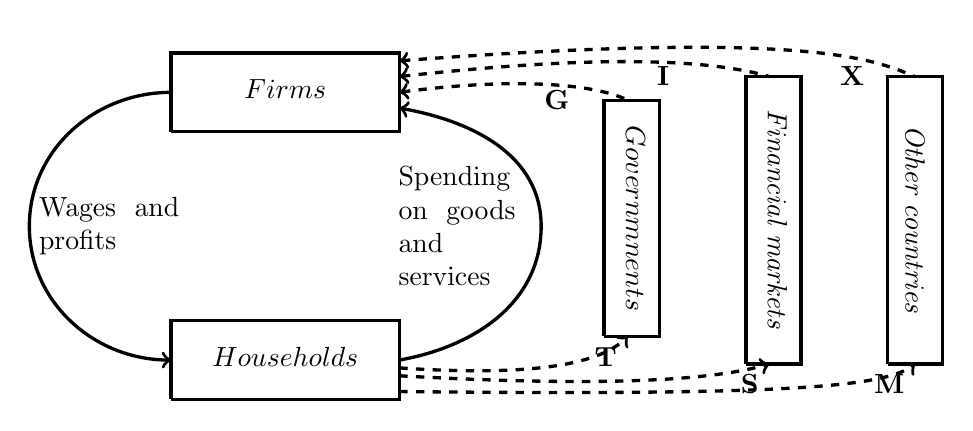
\begin{tikzpicture}[scale=1.0]
                    \draw[very thick](1.8, 0) --(4.7, 0) --(4.7, 1) --(1.8, 1) --(1.8, 0);
                    \draw[very thick](1.8, 3.4) --(4.7, 3.4) --(4.7, 4.4) --(1.8, 4.4) --(1.8, 3.4);
                    \draw[very thick](7.3, 0.8) --(8, 0.8) --(8, 3.8) --(7.3, 3.8) --(7.3, 0.8);
                    \draw[very thick](9.1, 0.45) --(9.8, 0.45) --(9.8, 4.1) --(9.1, 4.1) --(9.1, 0.45);
                    \draw[very thick](10.9, 0.45) --(11.6, 0.45) --(11.6, 4.1) --(10.9, 4.1) --(10.9, 0.45);
                    
                    \draw [very thick, ->](1.8, 3.9) to [out=-180, in=90](0, 2.2) to [out=-90, in=180](1.8, 0.5);
                    \draw [very thick, ->](4.7, 0.5) to [out=10, in=-90](6.5, 2.2) to [out=90, in=-10](4.7, 3.7); 
                    
                    \draw [very thick, ->] [dashed](4.7, 0.4) ..controls(6.2, 0.3) and(7.2, 0.4) ..(7.6, 0.8) node [below left] {$\textbf{T}$}; 
                    \draw [very thick, ->] [dashed](4.7, 0.3) ..controls(7.4, 0.15) and(8.7, 0.25) ..(9.4, 0.45) node [below left] {$\textbf{S}$};
                    \draw [very thick, ->] [dashed](4.7, 0.1) ..controls(9.55, 0.05) and(10.85, 0.15) ..(11.25, 0.45) node [below left] {$\textbf{M}$};			
                    
                    \draw [very thick, <-] [dashed](4.7, 3.9) ..controls(6.2, 4.1) and(7.2, 4) ..(7.6, 3.8); 
                    \draw [very thick, <-] [dashed](4.7, 4.1) ..controls(7.4, 4.4) and(8.7, 4.3) ..(9.4, 4.1);
                    \draw [very thick, <-] [dashed](4.7, 4.3) ..controls(10, 4.7) and(10.75, 4.3) ..(11.25, 4.1);
                    
                    \node [above] at(3.25, 0.3) {$Households$}; 
                    \node [above] at(3.25, 3.7) {$Firms$};
                    \node [below] at(6.7, 4.05) {$\textbf{G}$}; 
                    \node [below] at(8.05, 4.35) {$\textbf{I}$}; 
                    \node [below] at(10.45, 4.35) {$\textbf{X}$}; 
                    \node at(7.7, 2.3){\rotatebox{-90}{$Governmnents$}}; 
                    \node at(9.5, 2.275){ \rotatebox{-90}{\textit{Financial markets}}}; 
                    \node at(11.25, 2.275){ \rotatebox{-90}{\textit{Other countries}}}; 
                    
                    \node at(0, 2.2) [align = left, right] {Wages \ and \\ profits}; 
                    
                    \node at(6.3, 2.2) [align = left, left] {Spending \\ on \ goods \\ and \\ services};
                    \end{tikzpicture}
                \end{center}
                \caption{Narayanan, Adithya. \textit{Circular Flow of Income}.}
            \end{figure}
            Increases in fiscal expenditure, injections of 3 trillion Yuan, via monetary policies such as quantitative easing, and increases in business lending by 800 billion Yuan, part of the fiscal policy that the Chinese government has implemented, aims at increasing G. An eventual multiplier effect, ``a Keynesian theory that suggests a change in initial gov’t spending(G) will eventually have a greater(multiplied) effect on aggregate demand(AD), and hence on real GDP''(Ashton), on the economy is likely to occur, allowing the economy to exit the recession that is likely to occur in the short run, with the likely effect being an inflationary gap in the long run.
        \subsection{Policies implemented to assist firms:}
            The suspension of requirements to pay the civil aviation development fund assists the aviation industry, due to strict travel restrictions reducing demand, and as such the revenues and profits of aviation firms. Reductions in electricity prices for firms by 5\% assists in reducing a major cost of production for firms, thus assisting them. Allowing firms to halt pension fund payments for employees reduces a fixed cost that firms have to pay. Allowing loan repayments to be postponed reduces the short term burden on firms, however may increase the amount that will need to be paid in the long term. The implementation of such policies helps firms cope with the current situation.
        \subsection{Policies implemented to boost consumer confidence and expenditure:}
            The exemption of industries such as transport from Value-Added-Taxes(VAT), increases the disposable income left for consumers. As consumers face a greater tax burden due to inelastic demand, the removal of VAT assists consumers more than firms. Greater disposable income would likely encourage expenditure for other goods and services. The distribution of 300 million Yuan worth of vouchers assists consumers who may be struggling to meet their needs or to in general boost consumer expenditure, by increasing consumer disposable income. Aimed at specifically those struggling to meet needs, the doubling of temporary monthly allowance for low-income families ensures those who are struggling to meet their needs are assisted. The provision of unemployment benefits to vulnerable migrant workers allows the Chinese economy to assist likely frictionally unemployed individuals over the duration of the pandemic.
        \subsection{Policies intended to halt the spread of COVID-19:}
            The construction of temporary hospitals for COVID-19, assists to front line medical staff and most importantly the lockdowns are methods by which the government is halting the spread of COVID-19, in order to allow the economy to tackle the root cause of this issue. Direct resolution of this issue would assist in a quick recovery for the economy,as halting the spread of the virus would reduce. As such measures to reduce the impact of the pandemic on the labour force is the best way to ensure the shrinkage in the productive capacity of the economy remains minimal.
        \subsection{Conclusion:}
            The implementation of various policies assist different stakeholders with coping with the situation and their effectiveness can clearly be observed as China slowly recovers from the pandemic, as such the validity of economic theory is observed here with the policies implemented being effective.
        \subsection{Bibliography:}
        Ashton, Adam. 4.3 \textit{Fiscal Policy (Part 1)}. Adam Ashton.
        

        \hangindent=0.7cm
        \noindent
        Tang, Frank. “What Measures Has China Used to Combat the Economic Impact of Covid-19?” \textit{South China Morning Post}, 8 May 2020, www.scmp.com/economy/china-economy/article/308-3268/china-coronavirus-stimulus-what-measures-have-been-used. Accessed 10 May 2020.
        
        \hangindent=0.7cm
        \noindent
        Tragakes, Ellie. \textit{Economics for the IB Diploma}. Brantford, Ontario, W. Ross Macdonald School Resource Services Library, 2017.
        
        ‌


\end{document} 